%\VignetteIndexEntry{User manual}

\documentclass[nojss]{jss}

\usepackage[utf8]{inputenc}  
\usepackage[T1]{fontenc}
\usepackage{amsmath}
%% Set PDF 1.5 and compression, including object compression
%% Needed for MiKTeX -- most other distributions default to this
\ifx\pdfoutput\undefined
\else
  \ifx\pdfoutput\relax
  \else
    \ifnum\pdfoutput>0
      % PDF output
      \pdfminorversion=5
      \pdfcompresslevel=9
      \pdfobjcompresslevel=2
    \fi
  \fi
\fi
\usepackage{url}

%% for those who use Sweave please include the following line (with % symbols):
%% need no \usepackage(Sweave.sty)
% Vignette only: replace () by {} around Sweave.sty and uncomment the following line 
\usepackage[labelfont=bf, labelsep=period, justification=justified]{caption}

%%%%%%%%%%%%%%%%%%%%%%%%%%%%%%
%% declarations for jss.cls %%
%%%%%%%%%%%%%%%%%%%%%%%%%%%%%%

%% almost as usual
\author{Eric Marcon\\AgroParisTech\\UMR EcoFoG\And
        Stéphane Traissac\\AgroParisTech\\UMR EcoFoG\And
        Florence Puech\\RITM, Univ. Paris-Sud\\Université Paris-Saclay \& EXCESS\AND
        Gabriel Lang\\AgroParisTech\\ UMR 518 Math. Info. Appli\\
}

\title{Tools to Characterize Point Patterns: \pkg{dbmss} for \proglang{R}}

%% for pretty printing and a nice hypersummary also set:
\Plainauthor{Eric Marcon, Stéphane Traissac, Florence Puech, Gabriel Lang} %% comma-separated
\Plaintitle{Tools to Characterize Point Patterns: dbmss for R} %% without formatting
\Shorttitle{\pkg{dbmss} Package for R} %% a short title (if necessary)

%% an abstract and keywords
\Abstract{
The \pkg{dbmss} package for \proglang{R} provides an easy-to-use toolbox to characterize the spatial structure of point patterns.
Our contribution presents the state of the art of distance-based methods employed in economic geography, also used in ecology.
Topographic functions such as Ripley's \emph{K}, absolute functions such as Duranton and Overman's $K_d$ and relative functions such as Marcon and Puech's \emph{M} are implemented.
Their confidence envelopes (including global ones) and tests against counterfactuals are included in the package.
}
\Keywords{point patterns, spatial structure, \proglang{R}}
\Plainkeywords{point patterns, spatial structure, R} %% without formatting

\Address{
  Eric Marcon\\
  AgroParisTech, UMR EcoFoG\\
  Campus agronomique, BP 316\\
  97310 Kourou, French Guiana\\
  E-mail: \email{Eric.Marcon@ecofog.gf}\\

  Stéphane Traissac\\
  AgroParisTech, UMR EcoFoG\\
  Campus agronomique, BP 316\\
  97310 Kourou, French Guiana\\
  E-mail: \email{Stephane.Traissac@ecofog.gf}\\

  Florence Puech\\
  RITM\\
  Univ. Paris-Sud, Université Paris-Saclay\\
  92330 Sceaux, France\\
  E-mail: \email{Florence.Puech@u-psud.fr}\\

  Gabriel Lang\\
  AgroParisTech, INRA, UMR 518 Math. Info. Appli.\\
  16 rue Claude Bernard\\
  75005 Paris, France\\
  E-mail: \email{Gabriel.Lang@agroparistech.fr}\\

}

%% end of declarations %%%%%%%%%%%%%%%%%%%%%%%%%%%%%%%%%%%%%%%%%%%%%%%


\usepackage{Sweave}
\begin{document}
\input{dbmss-concordance}


\section{Introduction}
Characterizing spatial distributions of objects concerns numerous researchers in various fields. Amongst many questions, ecologists have been addressing the spatial attraction between species \citep{Duncan1991} or the non-independence of the location of dead trees in a forest \citep{Haase1997}. Analyzing the spatial distribution of plants, economists may be concerned by the location of new entrants \citep{Duranton2008} or by the location of shops according to the types of good sold \citep{Picone2009}. In epidemiology, researchers want to identify the spatial distribution of sick individuals in comparison to the population \citep{Diggle1991}. In these fields of research, the point process theory undoubtedly helps dealing with these questions. Exploratory statistics of point patterns widely rely on Ripley's seminal work \citep{Ripley1976, Ripley1977}, namely the \emph{K} function. A recent review of similar methods has been made by \cite{Marcon2012a} who called them distance-based measures of spatial concentration. We will write spatial structures here since both dispersion and concentration can be characterized. They are considered as novel and promising tools in spatial economics \citep{Combes2008}. The traditional approach to detect localization, \emph{i.e.}\ the degree of dissimilarity between the geographical distribution of an industry and that of a reference \citep{Hoover1936}, relies on discrete space (a country is divided in regions for example) and measures of inequality between zones, such as the classical Gini \citeyearpar{Gini1912} index or the more advanced Ellison and Glaeser \citeyearpar{Ellison1997} index. This approach suffers several limitations, mainly the Modifiable Areal Unit Problem (MAUP): results depend on the way zones are delimited and on the scale of observation \citep{Openshaw1979}. Distance-based methods have the advantage to consider space as continuous, \emph{i.e.}\ without any zoning, allowing detecting spatial structures at all scales simultaneously and solve MAUP issues.

These methods estimate the value of a function of distance to each point calculated on a planar point pattern, typically objects on a map. They all consist in counting \emph{neighbors} (up to or exactly at the chosen distance) around each \emph{reference point} and transform their number into a meaningful statistic. There are basically three possible approaches: just count neighbors, count neighbors per surface area or calculate the proportion of neighbors of interest among all neighbors. They define the three families of functions: absolute (how many neighbors are there?), topographic (how many neighbors per unit of area?) and relative (what is the ratio of neighbors of interest?). The function values are not the main motivation. The purpose is rather to test the point pattern against the null hypothesis that it is a realization of a known point process which does not integrate a property of interest. The basic purpose of Ripley's \emph{K} is to test the observed point pattern against complete spatial randomness (CSR), \emph{i.e.}\ a homogeneous Poisson process, to detect dependence between point locations (the null hypothesis supposes independent points) assuming homogeneity (\emph{i.e.}\ the probability to find a point is the same everywhere). Ripley-like functions, available in the proposed \pkg{dbmss} package, can be classified in three families:
\begin{itemize}
\item Topographic measures such as \emph{K} take space as their reference. They have been widely used in ecology \citep{Fortin2005}. They have been built from the point process theory and have a strong mathematical background.
\item Relative measures such as \emph{M} \citep{Marcon2010} compare the structure of a point type to that of another type (they can be considered as cases and controls). They have been developed in economics, where comparing the distribution of a sector of activity to that of the whole economic activity is a classical approach \citep{Combes2008}, but introduced only recently in ecology \citep{Marcon2012b}.
\item Absolute functions such as $K_d$ \citep{Duranton2005} have no reference at all but their value can be compared to the appropriate null hypothesis to test it.
\end{itemize}

Relative and absolute functions have been built from descriptive statistics of point patterns, not related to the underlying point processes, so they are seen as heuristic and ignored by the statistical literature \citep{Illian2008}. Topographic functions are implemented in the \pkg{spatstat} package \citep{Baddeley2005} for \proglang{R} \citep{R2012} but absolute and relative functions are missing. We fill this gap by proposing the \pkg{dbmss} package. It makes the computation of the whole set of distance-based methods simple for empirical researchers by introducing measures that are not available elsewhere and wrapping some topographic measures available in \pkg{spatstat} so that all can be used the same way.

Estimated values of the functions must be tested against a null hypothesis. The usual empirical way to characterize a spatial structure consists in computing the appropriate function and comparing it to the quantiles of a large number of simulations of the null hypothesis to reject \citep{Kenkel1988}. We propose extended possibilities to evaluate confidence envelopes, including ``global envelopes" \citep{Duranton2005}, a goodness-of-fit test \citep{Diggle1983} and an analytical test \citep{Lang2010, Marcon2013}.

Definitions of all functions and formulas for their estimation can be found in \cite{Marcon2012a} and are not repeated here, but they are summarized in the statistical background section. Their implementation is presented in the package content section.


\section{Rationale and statistical background}
We consider a map of points which often represents establishments in economic geography or trees in vegetation science. These points have two marks: a type (an industrial sector, a species...) and a weight (a number of employees, a basal area...). We want to apply to this point pattern a variety of exploratory statistics which are functions of distance between points, able to test the null hypothesis of independence between point locations. These functions are either topographic, absolute or relative. They can be interpreted as the ratio between the observed number of neighbors and the expected number of neighbors if points where located independently from each other. 
If reference and neighbor points are of the same type, the functions are univariate, to study concentration or dispersion. They are bivariate if the types differ, to address the colocation of types.
We detail this approach below.


\subsection{Topographic, homogeneous functions}
Topographic, homogeneous functions are Ripley's \emph{K} and its derivative \emph{g}. Their null hypothesis is a Poisson homogeneous process: rejecting it means that the process underlying the observed pattern is either not homogeneous or not independent. These functions are applied when homogeneity is assumed so independence only is tested by comparing the observed values of the function to their confidence envelope under CSR. Bivariate functions are tested against the null hypothesis of random labeling (points locations are kept unchanged but marks are redistributed randomly) or population independence (the reference point type is kept unchanged, the neighbor point type is shifted) following \cite{Goreaud2003}. The random labeling hypothesis considers that points preexist and their marks are the result of a process to test (\emph{e.g.}\ are dead trees independently distributed in a forest?). The population independence one considers that points belong to two different populations with their own spatial structure and wants to test whether they are independent from each other.

Edge effect correction is compulsory to compute topographic functions: points located close to boundaries have less neighbors because of the lack of knowledge outside the observation window. The \pkg{spatstat} package provides corrections following \cite{Ripley1988}, we use them.


\subsection{Topographic, inhomogeneous functions}
$K_{inhom}$ \citep{Baddeley2000} is the generalization of \emph{K} to inhomogeneous processes: it tests independence of points assuming the intensity of the process is known. Empirically, it generally has to be estimated from the data after assumptions on the way to do it relying on the theoretical knowledge of the process. The null hypothesis (``random position") is that the pattern comes from an inhomogeneous Poisson process of this intensity, which can be simulated. Applying $K_{inhom}$ to a single point type allows using the ``random location" null hypothesis, following \cite{Duranton2005}: observed points (with their marks) are shuffled among observed locations to test for independence. Bivariate $K_{inhom}$ null hypotheses may be random labeling or population independence as defined by \cite{Marcon2010}: reference points are kept unchanged, other points are redistributed across observed locations.

$K_{mm}$ \citep{Penttinen2006, Penttinen1992} generalizes \emph{K} to weighted points (weights are continuous marks of the points). Its null hypothesis in \pkg{dbmss} is random location. \cite{Penttinen1992} inferred the point process from the point pattern, and used the inferred process to simulate the null hypothesis patterns. This requires advanced spatial statistics techniques and knowledge about the process that is generally not available. The random location hypothesis is a way to draw null patterns simply, but ignoring the stochasticity of the point process.

The \emph{D} \citep{Diggle1991} function compares the \emph{K} function of points of interest (cases) to that of other points (controls). Its null hypothesis is random labeling.


\subsection{Absolute functions}\label{Absolute}
In their seminal paper, Duranton and Overman \citep{Duranton2005} study the distribution of industrial establishments in Great Britain.
Every establishment, represented by a point, is characterized by its position (geographic coordinates), its sector of activity (point type) and its number of employees (point weight).
The $K_d$ function \citep{Duranton2005} is the probability density to find a neighbor a given distance apart from a point of interest in a finite point process.
The $K^{emp}$ function integrates the weights of points: it is the density probability to find an employee $r$ apart from an employee of interest.

$K_d$ and $K^{emp}$ are absolute measures since their value is not normalized by the measure of space or any other reference: for a binomial process, $K_d$ increases proportionally to $r$ if the window is large enough to ignore edge effects \citep[the probability density is proportional to the perimeter of the circle of radius $r$,][]{Thomas2013}, then edge effects make it decrease to 0 when $r$ becomes larger than the window's size: it is a bell-shaped curve.
$K_d$ values are not interpreted but compared to the confidence envelope of the null hypothesis, which is random location.
Bivariate functions null hypotheses are random labeling, following \cite{Duranton2005}, \emph{i.e.}\ point types are redistributed across locations while weights are kept unchanged, or population independence (as for $K_{inhom}$).
It is not corrected for edge effects.
$K_d$ was designed to characterize the spatial structure of an economic sector, comparing it to the distribution of the whole activity.
From this point of view, it has been considered as a relative function \cite{Marcon2010}. 
We prefer to be more accurate and distinguish it from strict relative functions which directly calculate a ratio or a difference between the number of points of the type of interest and the total number of points.
What makes it relative is only its null hypothesis: changing it for random location (that of univariate $K_{inhom}$) would make univariate $K_d$ behave as a topographic function (testing independence of the distribution supposing its intensity is that of the whole activity).

$K_d$ is a leading tool in spatial economics. A great number of its applications can be found in the literature that confirms the recent interest for distance-based methods in spatial economics. A recent major study can be found in \cite{Ellison2010}.


\subsection{Relative functions}\label{Relative}

The univariate and bivariate \emph{M} function \citep{Marcon2010} are the ratio of neighbors of interest up to distance $r$ normalized by its value over the whole domain. Their null hypotheses are the same as $K_d$'s. They do not suffer edge effects. \cite{Marcon2010} show that the $M$ function respect most of the axioms generally accepted as the ``good properties'' to evaluate geographic concentration in spatial economics \citep{Combes2004, Duranton2005}.

\emph{m} \citep{Lang2014} is the density function measuring the same ratio as \emph{M}, at distance $r$.


\subsection{Unification}
Empirically, all estimators can be seen as variations in a unique framework: neighbors of each reference point are counted, their number is averaged and divided by a reference measure. Last, this average local result is divided by its reference value, calculated over the whole point pattern instead of around each point.

Choosing reference and neighbor point types allows defining univariate or bivariate functions, counting neighbors up to or at a distance defines cumulative or density functions, taking an area or a number of points as the reference measure defines topographic or relative functions. These steps are detailed for two functions to clarify them: we focus on Ripley's \emph{g} and Marcon and Puech's \emph{M} bivariate function. See \cite{Marcon2012a} for a full review.

Reference points are denoted $x_i$, neighbor points are $x_j$. For density functions such as \emph{g}, neighbors of $x_i$ are counted at a chosen distance $r$:

\begin{equation}
   n\left(x_i,r\right){\rm =}\sum_{j{\rm ,\ }i\ne j}{k\left(\left\|x_i{\rm -}x_j\right\|,r\right)c\left(i,j\right)}
\end{equation}

$k(\left\|x_i{\rm -}x_j\right\|,r)$ is a kernel estimator, necessary to evaluate the number of neighbors at distance $r$, and $c(i,j)$ is an edge-effect correction (points located close to boundaries have less neighbors because of the lack of knowledge outside the observation window).

To compute the bivariate \emph{M} function, reference points are of a particular type in a marked point pattern: $x_i \in \mathcal{R}$, where $\mathcal{R}$ is the set of points of the reference type. Neighbors of the chosen type are denoted $x_j \in \mathcal{N}$. In cumulative functions such as \emph{M}, neighbors are counted up to $r$:

\begin{equation}
   n\left(x_i,r\right){\rm =}\sum_{x_j \in \mathcal{N}, i \ne j}{{\mathbf 1}\left(\left\|x_i{\rm -}x_j\right\|\le r\right)w\left(x_j\right)}
\end{equation}

Points can be weighted, $w(x_j)$ is the neighbor's weight.

The number of neighbors is averaged then. $n$ is the number of reference points:

\begin{equation}
  \bar{n}\left(r\right)=\frac{1}{n}\sum_i{n\left(x_i,r\right)}
\end{equation}

The average number of neighbors is compared to a reference measure. It may be a measure of space (the perimeter of the circle of radius $r$ for \emph{g}), defining topographic functions:

\begin{equation}
  z\left(r\right)=2 \pi r
\end{equation}

It may also be the number of neighbors of all types in a relative function such as \emph{M}:

\begin{equation}
  z\left(r\right)=\sum_{j,i\ne j}{{\mathbf 1}\left(\left\|x_i{\rm -}x_j\right\|\le r\right)w\left(x_j\right)}
\end{equation}

Finally, $\frac{\bar{n}(r)}{z(r)}$ is compared to the same ratio computed on the whole window. For \emph{g}:

\begin{equation}
   \frac{\bar{n}_0}{z_0}{\rm =}\frac{n-1}{A}
\end{equation}

$A$ is the area of the window, $\bar{n}_0$ and $z_0$ are the limit values of $\bar{n}(r)$ and $z(r)$ when $r$ gets larger than the window's size. For \emph{M}, it comes:

\begin{equation}
   \frac{{\bar{n}}_0}{z_0}=\frac{1}{n}\sum_i{\frac{W_\mathcal{N}}{W-w\left(x_i\right)}}
\end{equation}

$W_\mathcal{N}$ is the total weight of neighbor points, $W$ that of all points. Finally, despite the functions are quite different (density vs.\ cumulative, topographic vs.\ relative, univariate vs.\ bivariate), both estimators can be written as ${\frac{{\bar{n}}}{z}}/{\frac{{\bar{n}}_0}{z_0}}$. Their value (except for absolute functions) can be interpreted as a location quotient: $g(r)=2$ or $M(r)=2$ means than twice more neighbors are observed at (or up to) distance $r$ than expected on average, \emph{i.e.}\ ignoring the point locations in the window. The appropriate function will be chosen among the toolbox according to the question raised.


\section{Package content}

The \pkg{dbmss} package contains a full (within the limits of the literature reviewed in section 2) set of functions to characterize the spatial structure of a point pattern, including tools to compute the confidence interval of the counterfactual.
It allows addressing big datasets thanks to \proglang{C++} code used to calculate distances between pairs of points \citep[using \pkg{Rcpp} and \pkg{RcppParallel} infrastructure][]{Eddelbuettel2011, Allaire2015}. Computational requirements actually are an issue starting from say 10,000 points \citep[see][for instance]{Ellison2010}. Memory requirement is $O(n)$, \emph{i.e.}\ proportional to the number of points to store their location and type. We use loops to calculate distances and increment summary statistics rather than store a distance matrix which is $O(n^2)$, following \cite{Scholl2013}. Computation time is $O(n^2)$ because $n(n-1)/2$ pair distances must be calculated.

We consider planar points patterns (sets of points in a 2-dimensional space) with marks of a special kind: each point comes with a continuous mark (its weight) and a discrete one (its type). We call this special type of point pattern ``weighted, marked, planar point patterns'' and define objects of class \code{wmppp}, which derives from \code{ppp} class as defined in \pkg{spatstat}. Marks are a dataframe with two columns, \code{PointWeight} containing the weights of points, and \code{PointTypes} containing the types, as factors.

A \code{wmppp} object can be created by the \code{wmppp()} function which accepts a dataframe as argument, or converted from a \code{ppp} object by \code{as.wmppp()}. Starting from a csv file containing point coordinates, their type and their weight in four columns, a \code{wmppp} object can be created by just reading the file with \code{read.csv()} and applying \code{wmppp()} to the result. Options are available to specify the observation window or guess it from the point coordinates and set default weights or types to points when they are not in the dataframe, see the package help for details. The simplest code to create a \code{wmppp} with 100 points is as follows. It draws point coordinates between 0 and 1, and creates a \code{wmppp} with a default window, all points are of the same type named ``All" and their weight is 1.


\begin{Schunk}
\begin{Sinput}
R> Pattern <- wmppp(data.frame(X = runif(100), Y = runif(100)))
R> summary(Pattern)
\end{Sinput}
\begin{Soutput}
Marked planar point pattern:  100 points
Average intensity 103.9027 points per square unit

Coordinates are given to 8 decimal places

Mark variables: PointWeight, PointType
Summary:
  PointWeight PointType
 Min.   :1    All:100  
 1st Qu.:1             
 Median :1             
 Mean   :1             
 3rd Qu.:1             
 Max.   :1             

Window: rectangle = [0.0089494, 0.978967] x [0.0001234, 0.9923104] 
units
Window area = 0.962439 square units
\end{Soutput}
\end{Schunk}

\subsection{Distance-based functions}
All functions are named \code{Xhat} where \code{X} is the name of the function: 
Ripley's \emph{g} and \emph{K}, and \emph{K}'s normalization, Besag's \emph{L} \citeyearpar{Besag1977}; 
Penttinen's $K_{mm}$ and $L_{mm}$; 
Diggle and Chetwynd's \emph{D}; 
Baddeley et al.'s $K_{inhom}$ and its derivative $g_{inhom}$; 
Marcon and Puech's \emph{M}
and Duranton and Overman's $K_d$ (including its weighted version $K^{emp}$). The suffix \code{hat} has been used to avoid confusion with other functions in \proglang{R}: \code{D} exists in the \pkg{stats} package for example.
Arguments are:
\begin{itemize}
\item A weighted, marked planar point pattern (a \code{wmppp} class object). The window can be a polygon or a binary image, as in \pkg{spatstat}.
\item A vector of distances.
\item Optionally a reference and a neighbor point type to calculate bivariate functions, or equivalently the types of cases and controls for the \emph{D} function.
\item Some optional arguments, specific to some functions.
\end{itemize}

Topographic functions require edge-effect corrections, provided by \pkg{spatstat}: the \code{best} correction is systematically used. Relative functions ignore the window. Technical details are provided in help files.

These functions return an \code{fv} object, as defined in \pkg{spatstat}, which can be plotted.

\subsection{Confidence envelopes}

The classical confidence intervals, calculated by Monte-Carlo simulations \citep{Kenkel1988} are obtained by the \code{XEnvelope} function, where \code{X} is the function's name. Arguments are the number of simulations to run, the risk level, those of the function and the null hypothesis to simulate. These functions return a \code{dbmssEnvelope} object which can be plotted.

Null hypotheses have been discussed by \cite{Goreaud2003} for topographic functions such as \emph{K} and by \cite{Marcon2010} for relative functions. The null hypothesis for univariate functions is random position (points are drawn in a Poisson process for topographic functions) or random location (points are redistributed across actual locations for relative functions). Bivariate functions support random labeling and population independence null hypotheses. The possible values of arguments are detailed in the help file of each function.

Building a confidence envelope this way is problematic because the test is repeated at each distance. The underestimation of the risk has been discussed by \cite{Loosmore2006}. \cite{Duranton2005} proposed a global envelope computed by the repeated elimination of simulations reaching an extreme value at any distance until the desired level is reached. The argument \code{Global = TRUE} is used to obtain it instead of the local one.

\subsection{Examples}


\begin{figure}
\centering
\includegraphics{dbmss-Toulouse}
\caption{Map of emergencies in the urban area of Toulouse, France, during year 2004 (about 33~km from south to north). (a) 20,820 emergencies  have been recorded and mapped (many points are confused at the figure scale). (b) Locations of the 10 percent most serious ones.}
\label{Toulouse}
\end{figure}

We illustrate the main features of the package by two examples. The first one comes from the economic literature \citep{Bonneu2007}\footnote{The dataset can be downloaded from: 
 \url {http://publications-sfds.fr/index.php/csbigs/article/downloadSuppFile/376/69}}. A point pattern gathers data about 20,820 emergencies implying the fire department of the urban area around Toulouse, France, during the year 2004 (Figure~\ref{Toulouse}). The workload associated to each emergency (the number of men $\times$ hours it required) is known. The original study tested the dependence between workload and location of emergencies: it did not exclude the null hypothesis of random labeling. We have a complementary approach here: we consider the 10 percent more serious emergencies, \emph{i.e.}\ those which caused the highest workload. $K_d$ may detect concentration (or dispersion) if, at a distance $r$ from a serious emergency, the probability to find another serious emergency is greater (or lower) than that of finding an emergency whatever its workload:

\begin{Schunk}
\begin{Sinput}
R> load("CSBIGS.Rdata")
R> Category <- cut(Emergencies$M, quantile(Emergencies$M, 
+      c(0, 0.9, 1)), labels = c("Other", "Biggest"), include.lowest = TRUE)
R> X <- wmppp(data.frame(X = Emergencies$X, Y = Emergencies$Y, 
+      PointType = Category), win = Region)
R> X$window$units <- c("meter", "meters")
R> KdE <- KdEnvelope(X, r = seq(0, 10000, 100), NumberOfSimulations = 1000, 
+      ReferenceType = "Biggest", Global = TRUE)
R> plot(KdE, main = "")
\end{Sinput}
\end{Schunk}

The \code{Emergencies} data frame contains point coordinates (in meters) in columns \code{X} and \code{Y} and workload in column \code{M}. The second line of the code creates a vector containing a factor describing the workload to separate its 10\% higher values. A \code{wmppp} object is created then, containing the points and their mark. The \code{KdEnvelope} function is run from 0 to 10~km by steps of 100~m for the most serious emergencies. Figure~\ref{Kd} shows that the 10\% most serious emergencies are more dispersed than the distribution of all emergencies. This opens the way to discuss on the optimal location of fire stations.

\begin{figure}
\centering
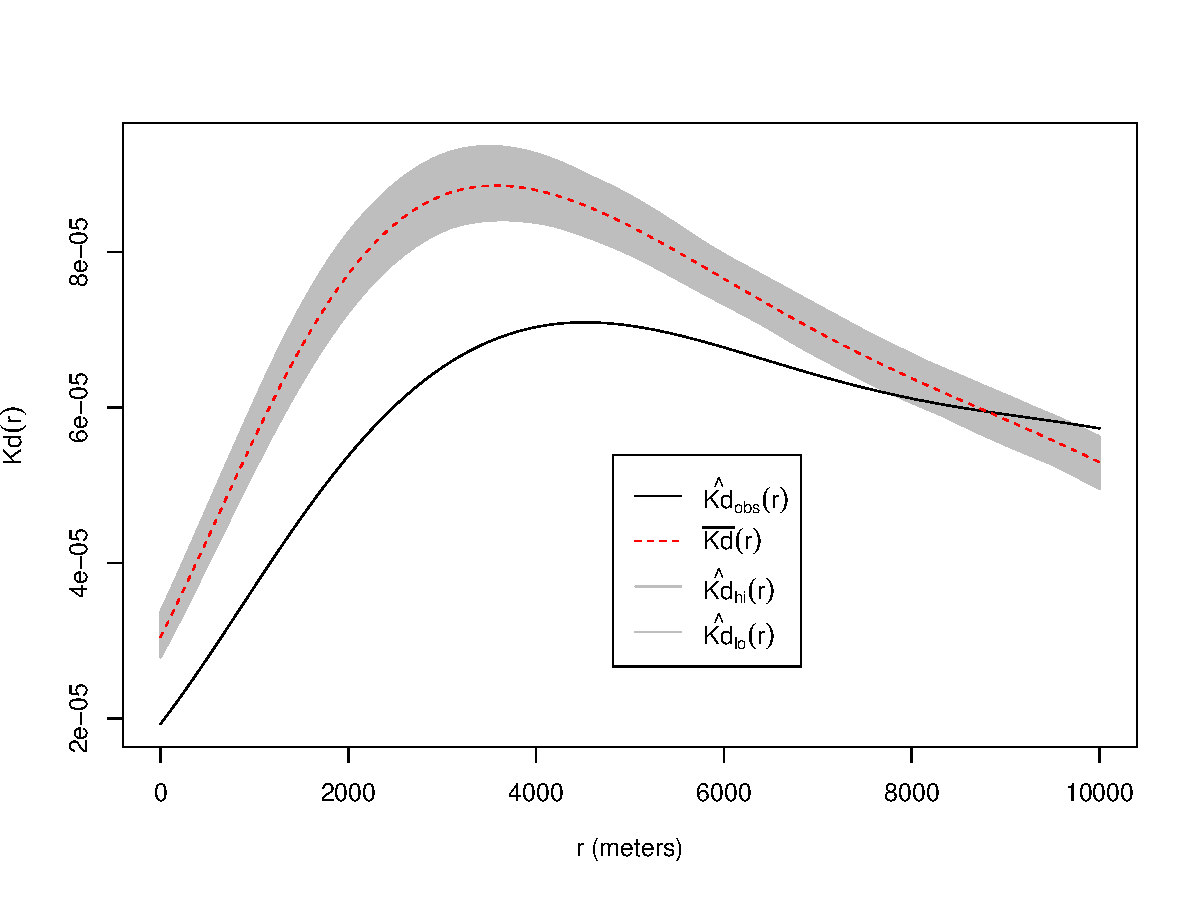
\includegraphics{KdFig.pdf}
%% Chunk not run to save CRAN resources. 
%% Comment the previous line and set eval=TRUE below to run it
\caption{Representation of $K_d(r)$ values of the 10\% most serious emergencies in year 2004 in Toulouse urban area, showing their significant dispersion at all distances up to 10~km. The solid, black curve is  $K_d$. The dotted red curve is the average simulated value and he shaded area is the confidence envelope under the null hypothesis of random location. The risk level is 5\%, 1000 simulations have been run. Distances are in meters.}
\label{Kd}
\end{figure}

The second example uses the \code{paracou16} point pattern (Figure~\ref{paracou16}) provided in the package. It represents the distribution of trees in a 4.1-ha tropical forest plot in the Paracou field station in French Guiana \citep{Gourlet2004}. It contains 2426 trees, whose species is either \emph{Qualea rosea}, \emph{Vouacapoua americana} or \emph{Other} (one of more than 300 species). Weights are basal areas (the area of the stems virtually cut 1.3 meter above ground), measured in square centimeters.

\begin{Schunk}
\begin{Sinput}
R> data("paracou16")
R> plot(paracou16, which.marks = "PointWeight", main = "", 
+      legend = FALSE)
\end{Sinput}
\end{Schunk}

\begin{figure}
\centering
\includegraphics{dbmss-P16Fig}
\caption{\code{paracou16} point pattern. Circles are centered on trees in a 4.1-ha forest plot (the containing rectangle is 200~m wide by 250~m long). Circle sizes are proportional to the basal areas of trees.}
\label{paracou16}
\end{figure}

The question to test is dependence between the distributions of the two species of interest.
Bivariate $M(r)$ is calculated for $r$ between 0 and 30 meters. 1000 simulations are run to build the global confidence envelope.

\begin{Schunk}
\begin{Sinput}
R> Envelope <- MEnvelope(paracou16, r = seq(0, 30, 2), NumberOfSimulations = 1000, 
+      Alpha = 0.05, ReferenceType = "V. Americana", NeighborType = "Q. Rosea", 
+      SimulationType = "RandomLabeling", Global = TRUE)
R> plot(Envelope, main = "", ylim = c(0, 20))
\end{Sinput}
\end{Schunk}

\begin{figure}
\centering
\includegraphics{dbmss-MFig}
\caption{Representation of $M(r)$ values of \emph{Qualea rosea} around \emph{Vouacapoua Americana} trees in the \code{paracou16} point pattern. The solid, black curve is \emph{M}. The dotted red curve is the average simulated value. The shaded area is the confidence envelope. $M=1$ is expected if points are independently distributed. The risk level is 5\%, 1000 simulations have been run. Distances are in meters.}
\label{MQr}
\end{figure}

The calculated function (Figure~\ref{MQr}) is \emph{M}, showing the repulsion between \emph{V. Americana} and \emph{Q. rosea} up to 30 m. Significance is unclear, since the observed values of the function are very close to the lower bound of the envelope. The complete study, with a larger dataset allowing significant results, can be found in \cite{Marcon2012b}.

\subsection{Goodness-of-fit test}
A Goodness-of-fit test for \emph{K} has been proposed by \cite{Diggle1983}, applied to \emph{K} by \cite{Loosmore2006} and to \emph{M} by \cite{Marcon2012b}. It calculates the  distance between the actual values of the function and its average value obtained in simulations of the null hypothesis. The same distance is calculated for each simulated point pattern, and the returned $p$~value of the test if the ratio of simulations whose distance is larger than that of the real point pattern. The test is performed by the \code{GoFtest} function whose argument is the envelope previously calculated (actually, the function uses the simulation values). Applied to the example of Paracou trees, the $p$~value is:

\begin{Schunk}
\begin{Sinput}
R> GoFtest(Envelope)
\end{Sinput}
\begin{Soutput}
[1] 0.25
\end{Soutput}
\end{Schunk}

\subsection{Ktest}
The \emph{Ktest} has been developed by Lang and Marcon \citep{Lang2010, Marcon2013}. It does not rely on simulations and returns the $p$~value to erroneously reject complete spatial randomness (CSR) given the values of \emph{K}. It relies on the exact variance of \emph{K} calculated with edge-effect corrections. It only works in a rectangular window.

The following example tests a 1.5-ha subset of \code{paracou16} (100~m by 150~m, origin at the southwestern corner). It rejects CSR (p=0.0027).

\begin{Schunk}
\begin{Sinput}
R> data("paracou16")
R> RectWindow <- owin(c(300, 400), c(0, 150))
R> X <- paracou16[RectWindow]
R> Ktest(X, seq(5, 50, 5))
\end{Sinput}
\begin{Soutput}
[1] 0.002682576
\end{Soutput}
\end{Schunk}


\section{Conclusion}

We built this package to provide an easy-to-use toolbox for users of spatial statistics mainly in economic geography and ecology. We wrapped up some \pkg{spatstat} functions to allow using them similarly to our original functions to build a rather complete set of tools, including topographic, absolute and relative functions. The analysis is limited to testing a point pattern against an appropriate null hypothesis, according to the framework developed in the economic literature \citep{Combes2008} but we believe \pkg{dbmss} is a useful extension of \pkg{spatstat} for researchers who are motivated by empirical results more than by the tools themselves, whatever their scientific field. 
Full features for point pattern analysis can be found in \pkg{spatstat} for who wants to go further, including simulation of many point processes as alternate null hypotheses and model fitting beyond exploratory statistics.

Future developments include the use of distance matrices as input of the distance-based functions to allow addressing road distance or geographic coordinates. We will also develop subsampling techniques to be able to manage huge datasets (several million points) whose distances can not all be calculated in a reasonable time.


\section{Acknowledgments}

We thank Florent Bonneu who kindly allowed us to use his published fire emergency data.

\bibliography{dbmss}

\end{document}
